%! TEX root = ../main.tex

\titre{Intégration numérique}

Dans ce TP, on s'intéresse au problème du calcul numérique d'une intégrale \[
    I_{a, b}(f) = \int_{a}^{b} f(t)dt
\]
d'une fonction $ f $ continue sur le segment $ [a, b] $. Ce problème intervient régulièrement en physique, mathématiques, biologie, et d'autres domaines encore, lorsqu'il n'est pas possible de calculer une primitive de $ f $, même en ayant recours aux techniques de changements de variable, intégration par partie, et autres techniques d'intégration plus avancées.

Les méthodes que l'on considère se décomposent en deux étapes:
\begin{enumerate}
    \item Une méthode de base pour calculer $ \hat{I}_{u, v}(f) $ une approximation de l'intégrale sur un petit intervalle $ [u, v] $.
    \item Ensuite on utilise la relation de Chasles pour les intégrales: on considère une subdivision régulièrement espacée $ (u_0, u_1, \ldots, u_n) $ de $ [a, b] $ (voir \autoref{fig:subdivision-reguliere}) et on calcule \[
        \hat{I}^{(n)}_{a, b}(f) = \hat{I}_f(u_0, u_1) + \hat{I}_f(u_1, u_2) + \ldots + \hat{I}_f(u_{n-1}, u_n)
    \]
    C'est la généralisation dite \textit{composite} de la méthode de base.
\end{enumerate}

Les méthodes de base auxquelles nous allons nous intéresser sont dites des \textit{de quadrature}, c'est-à-dire qu'elles conduisent à approcher l'intégrale par une somme pondérée finie de valeurs de $ f $ évaluée en différents points. Autrement dit, les méthodes de base calculent une approximation de la forme 
\begin{equation}
    \label{eq:quadrature}
    \hat{I}_{u, v}(f) = (v-u) \cdot \sum_{k=0}^{p} \alpha_i f(x_i)
\end{equation}
où les poids $ \alpha_1, \ldots, \alpha_p $ sont des réels indépendants de $ f $, et les $ x_i $ sont des réels de l'intervalle $ [u, v] $.

L'erreur d'approximation est la différence entre $ I_{u, v}(f) $ et l'approximation de la méthode de base $ \hat{I}_{u, v}(f) $, soit \[
    E_{u, v}(f) =  I_{u, v}(f) -  \hat{I}_{u, v}(f) 
\]

L'erreur d'approximation composite est l'erreur pour l'approximation de la généralisation composite de la méthode de base, soit \[
    E^{(n)}_{a, b}(f) =  I_{a, b}(f) -  \hat{I}^{(n)}_{a, b}(f) 
\]


Enfin, on dira qu'une méthode \textrm{est d'ordre $ k $} lorsque l'erreur d'approximation est nulle si $ f $ est un polynôme de degré inférieur ou égal à $ k $.

On se donne ici la formule pour calculer le $ k $-ième point de la subdivision régulière de $ [a, b] $ de taille $ n $ \[
    u_k = a + k\frac{b-a}{n}, \quad k=0, \ldots, n
\]

\begin{figure}[h!]
    \centering
    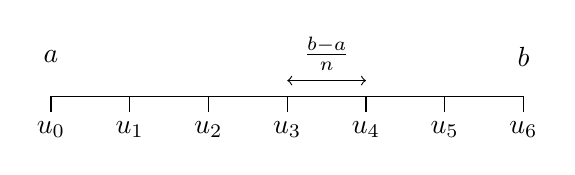
\begin{tikzpicture}
        % Segment
        \draw (0,0) -- (6,0);
        \node at (0,0.5) {$a$};
        \node at (6,0.5) {$b$};
        % Ticks and labels
        \foreach \x in {0,...,6}
        {
          \draw (\x,0) -- (\x,-0.2) node[below] {$u_{\x}$};
        }

        % Double-ended arrow
        \draw[<->] (3,0.2) -- (4,0.2) node[midway, above] {$\frac{b-a}{n}$};
    \end{tikzpicture}
    \caption{Subdivision régulière de $ [0, 1] $ de taille $ 5 $}
    \label{fig:subdivision-reguliere}
\end{figure}

\section{Méthode du rectangle}

\subsection{Méthode de base}
La méthode du rectangle est la plus simple : elle consiste à approcher la fonction par une unique valeur qu'elle prend (en général à une des extrêmités de l'intervalle). Ainsi, si l'on choisit l'extrêmité gauche, l'approximation s'écrit \[
    \hat{I}_{u, v}(f) = (v-u) \cdot f(u)
\]
Avec la terminologie vue plus haut, cela revient à prendre $ p=0 $, $ \alpha_0=1 $ et $ x_0=u $

\quessques Que devient la formule pour $ \hat{I}(u, v) $ si l'on choisit plutôt l'extrêmité droite ?
\ssques Quel est l'ordre de la méthode du rectangle si l'on choisit l'extrêmité gauche ? l'extrêmité droite ?

\begin{figure}[h!]
    \centering
    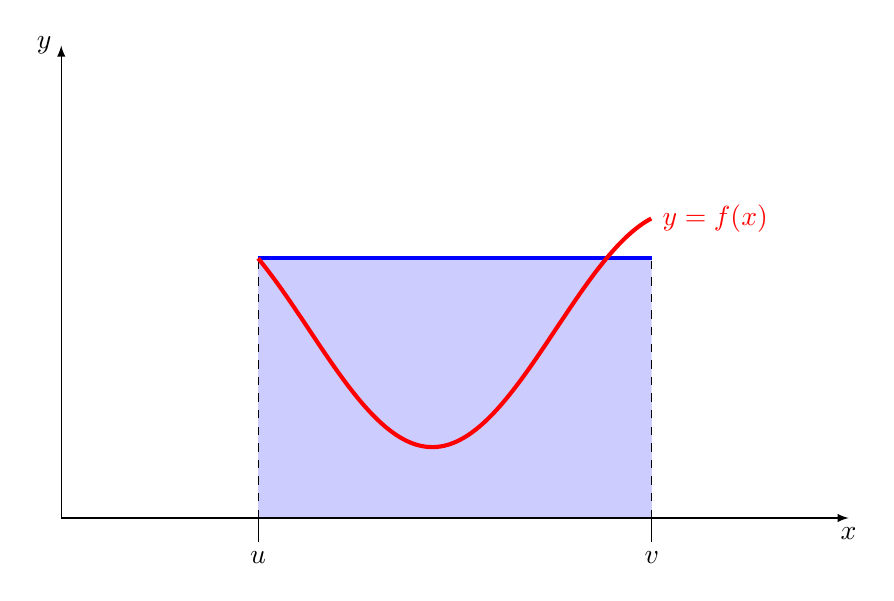
\begin{tikzpicture}[xscale=5, yscale=3]

        % Area under the constant function
        \fill[blue!20, domain=0.5:1.5, variable=\x]
            (0.5,0)
            -- plot ({\x}, {0.8+0.5*sin(deg(2.5))})
            -- (1.5,0)
            -- cycle;
        % Dotted vertical line
        \draw[dashed] (0.5,0) -- (0.5, {0.8+0.5*sin(deg(2.5)});
        \draw[dashed] (1.5,0) -- (1.5, {0.8+0.5*sin(deg(2.5)});

        % axis
        \draw[-latex] (0,0) -- (2,0) node[below] {$x$};
        \draw[-latex] (0,0) -- (0,2) node[left] {$y$};
        \draw (0.5,0) -- (0.5,-0.1) node[below] {$u$};
        \draw (1.5,0) -- (1.5,-0.1) node[below] {$v$};

        % Constant function
        \draw[blue, line width=1.5pt, domain=0.5:1.5] plot (\x, {0.8+0.5*sin(deg(2.5))});

        % Curve
        \draw[red, line width=1.5pt, domain=0.5:1.5, samples=100] plot (\x, {0.8+0.5*sin(deg(5*\x))}) node[right] {$y=f(x)$};
    \end{tikzpicture}
    \caption{Méthode du rectangle pour l'extrêmité gauche}
    \label{fig:rectangle-method}
\end{figure}

\quessques Écrire une fonction \texttt{rectangle(f, u, v)} qui prend comme argument une fonction \texttt{f}, et des bornes \texttt{u} et \texttt{v}, et renvoie l'approximation de l'intégrale de \texttt{f} entre \texttt{u} et \texttt{v} donnée par la méthode du rectangle. 
\ssques Tester la fonction avec $ \sin(x) $ entre $ 3 $ et $ 4 $. 
\ssques Calculer l'erreur pour l'exemple précédent.


\subsection{Méthode du rectangle composite}

La généralisation composite de la méthode du rectangle applique la méthode du rectangle à chaque subdivision de l'intervalle $ [a, b] $. En utilisant l'extrêmité gauche, cela s'écrit donc
\begin{align*}
    \hat{I}^{(n)}_{a, b}(f) &= \sum_{k=0}^{n-1} f(u_k)(u_{k+1}-u_k)\\
                          &= \frac{b-a}{n}\sum_{k=0}^{n-1} f(a + k \frac{b-a}{n}) 
\end{align*}

C'est essentiellement la forme d'une intégrale de Riemann !

\begin{figure}[h!]
    \centering
    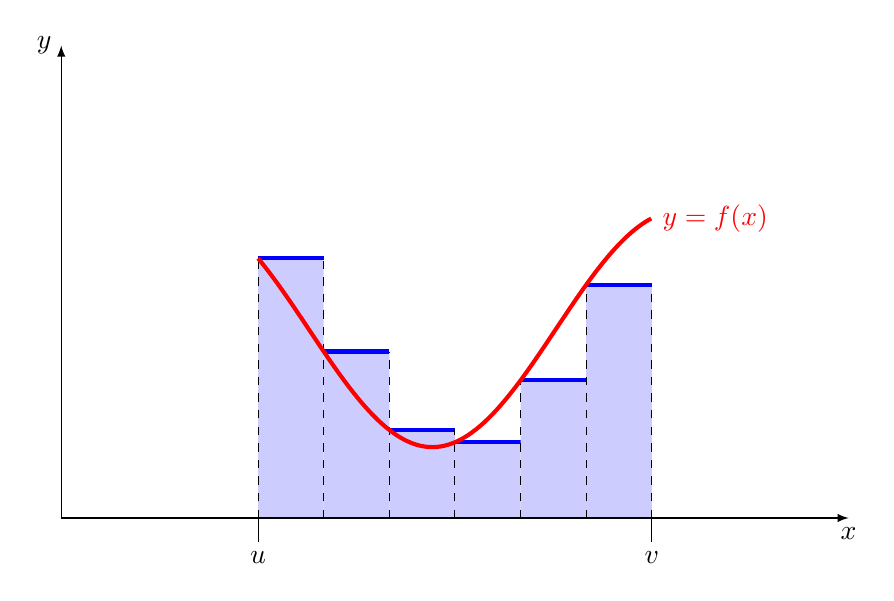
\begin{tikzpicture}[xscale=5, yscale=3]
        % Subdivisions and constant curves
        \foreach \i in {0,1,2,3,4,5} {
            \pgfmathsetmacro{\xa}{0.5 + \i*(1/6)}
            \pgfmathsetmacro{\xb}{0.5 + (\i+1)*(1/6)}
            \fill[blue!20, domain=\xa:\xb, variable=\x]
                (\xa,0) -- plot ({\x}, {0.8+0.5*sin(deg(5*\xa))}) -- (\xb,0) -- cycle;
            \draw[blue, line width=1.5pt, domain=\xa:\xb] plot (\x, {0.8+0.5*sin(deg(5*\xa))});
            \draw[dashed] (\xa,0) -- (\xa, {0.8+0.5*sin(deg(5*\xa))});
            \draw[dashed] (\xb,0) -- (\xb, {0.8+0.5*sin(deg(5*\xa))});
        }

        % Axis and ticks
        \draw[-latex] (0,0) -- (2,0) node[below] {$x$};
        \draw[-latex] (0,0) -- (0,2) node[left] {$y$};
        \draw (0.5,0) -- (0.5,-0.1) node[below] {$u$};
        \draw (1.5,0) -- (1.5,-0.1) node[below] {$v$};

        % Curve
        \draw[red, line width=1.5pt, domain=0.5:1.5, samples=100] plot (\x, {0.8+0.5*sin(deg(5*\x))}) node[right] {$y=f(x)$};

    \end{tikzpicture}

    \caption{Méthode composite du rectangle pour l'extrêmité gauche}
    \label{fig:rectangle-composite-method}
\end{figure}

\quessques Écrire une fonction \texttt{rectangle\_composite(f, a, b, n)} qui calcule l'approximation de l'intégrale de \texttt{f} entre \texttt{a} et \texttt{b} pour la méthode du rectangle composite, avec une subdivision de taille \texttt{n}. On pourra utiliser la fonction \texttt{np.linspace} (cherchez la documentation en ligne pour comprendre comment elle fonctionne).
\ssques Calculer l'erreur avec la même fonction test qu'avant, pour des subdivisions de taille $ 10 $, $ 100 $ et $ 1000 $.


\section{Méthode du point milieu}
\subsection{Méthode de base}

Une amélioration simple de la méthode du rectangle consiste à utiliser la valeur du milieu de l'intervalle, plutôt que celle d'une des extrêmités. Cela constitue la méthode du point milieu. Ainsi, la formule d'approximation de $ I_{u, v}(f) $ s'écrit \[
    \hat{I}_{u, v}(f) = (v-u)f(\frac{u+v}{2})
\]

\quessques Quel est l'ordre de la méthode du point milieu ?
\ssques Implémenter une fonction \texttt{point\_milieu(f, u, v)}. Calculer l'erreur avec la même fonction test que précédemment.


\begin{figure}[h!]
    \centering
    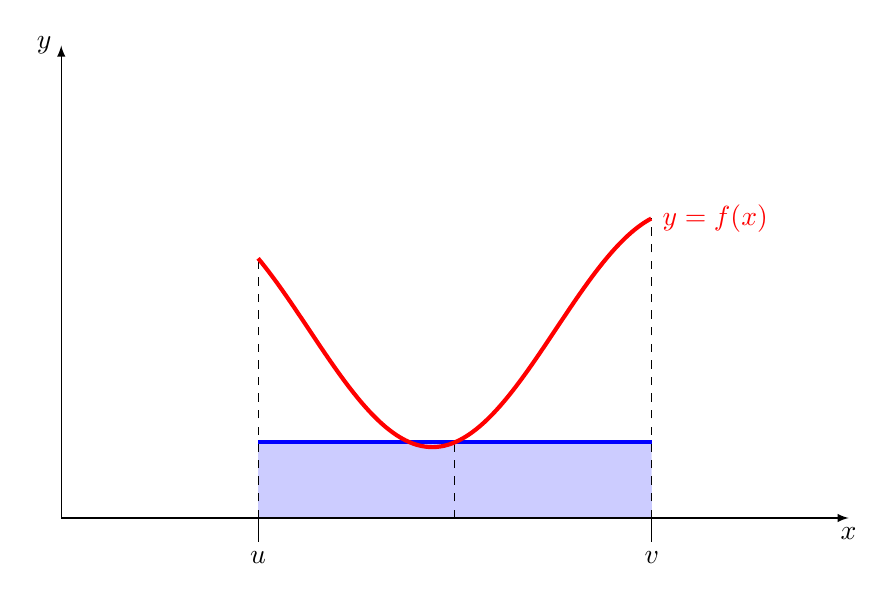
\begin{tikzpicture}[xscale=5, yscale=3]

        % Area under the constant function
        \fill[blue!20, domain=0.5:1.5, variable=\x]
            (0.5,0)
            -- plot ({\x}, {0.8+0.5*sin(deg(5))})
            -- (1.5,0)
            -- cycle;
        % Dotted vertical line
        \draw[dashed] (0.5,0) -- (0.5, {0.8+0.5*sin(deg(2.5)});
        \draw[dashed] (1,0) -- (1, {0.8+0.5*sin(deg(5)});
        \draw[dashed] (1.5,0) -- (1.5, {0.8+0.5*sin(deg(7.5)});

        % axis
        \draw[-latex] (0,0) -- (2,0) node[below] {$x$};
        \draw[-latex] (0,0) -- (0,2) node[left] {$y$};
        \draw (0.5,0) -- (0.5,-0.1) node[below] {$u$};
        \draw (1.5,0) -- (1.5,-0.1) node[below] {$v$};


        % Constant function
        \draw[blue, line width=1.5pt, domain=0.5:1.5] plot (\x, {0.8+0.5*sin(deg(5))});
        % Curve
        \draw[red, line width=1.5pt, domain=0.5:1.5, samples=100] plot (\x, {0.8+0.5*sin(deg(5*\x))}) node[right] {$y=f(x)$};
    \end{tikzpicture}
    \caption{Méthode du point milieu}
    \label{fig:point-milieu-method}
\end{figure}

\subsection{Méthode du point milieu composite}

La généralisation composite de la méthode du point milieu applique la méthode du point mileu à chaque subdivision de l'intervalle $ [a, b] $. Cela s'écrit 
\begin{align*}
    \hat{I}^{(n)}_{a, b}(f) &= \sum_{k=0}^{n-1} f(\frac{u_k+u_{k+1}}{2})(u_{k+1}-u_k)\\
                          &= \frac{b-a}{n}\sum_{k=0}^{n-1} f(a + (k+\frac{1}{2}) \frac{b-a}{n}) 
\end{align*}

\quessques Écrire une fonction \texttt{point\_milieu\_composite(f, a, b, n)} qui calcule l'approximation de l'intégrale de \texttt{f} entre \texttt{a} et \texttt{b} pour la méthode du point mileu composite, avec une subdivision de taille \texttt{n}.
\ssques Calculer l'erreur avec la même fonction test qu'avant, pour des subdivisions de taille $ 10 $, $ 100 $ et $ 1000 $. Comparez avec la méthode du rectangle.

\begin{figure}[h!]
    \centering
    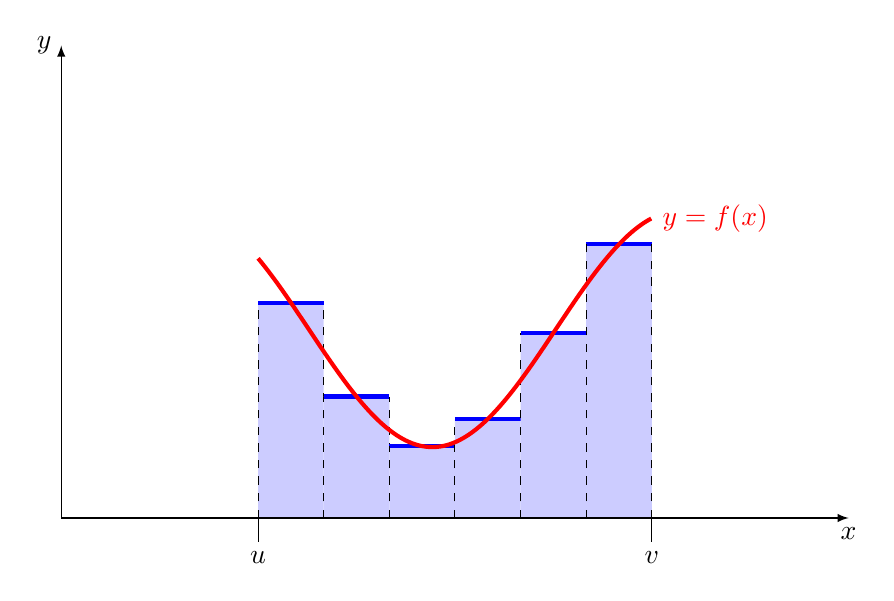
\begin{tikzpicture}[xscale=5, yscale=3]
        % Subdivisions and constant curves
        \foreach \i in {0,1,2,3,4,5} {
            \pgfmathsetmacro{\xa}{0.5 + \i*(1/6)}
            \pgfmathsetmacro{\xb}{0.5 + (\i+1)*(1/6)}
            \pgfmathsetmacro{\xmid}{(\xa+\xb)/2}
            \fill[blue!20, domain=\xa:\xb, variable=\x]
                (\xa,0) -- plot ({\x}, {0.8+0.5*sin(deg(5*\xmid))}) -- (\xb,0) -- cycle;
            \draw[blue, line width=1.5pt, domain=\xa:\xb] plot (\x, {0.8+0.5*sin(deg(5*\xmid))});
            \draw[dashed] (\xa,0) -- (\xa, {0.8+0.5*sin(deg(5*\xmid))});
            \draw[dashed] (\xb,0) -- (\xb, {0.8+0.5*sin(deg(5*\xmid))});
        }

        % Axis and ticks
        \draw[-latex] (0,0) -- (2,0) node[below] {$x$};
        \draw[-latex] (0,0) -- (0,2) node[left] {$y$};
        \draw (0.5,0) -- (0.5,-0.1) node[below] {$u$};
        \draw (1.5,0) -- (1.5,-0.1) node[below] {$v$};

        % Curve
        \draw[red, line width=1.5pt, domain=0.5:1.5, samples=100] plot (\x, {0.8+0.5*sin(deg(5*\x))}) node[right] {$y=f(x)$};

    \end{tikzpicture}

    \caption{Méthode composite du point milieu}
    \label{fig:point-milieu-composite-method}
\end{figure}


\section{Méthode du trapèze}
\subsection{Méthode de base}
La méthode du trapèze choisit de considérer que $ f $ n'est non plus constante sur l'intervalle $ [u, v] $ mais affine. Ainsi, avec cette méthode, on approxime $ I_{u,v}(f) $ par $ I_{u,v}(\hat{f}) $ où $ \hat{f} $ est l'approximation affine de $ f $ sur $ [u, v] $, c'est-à-dire que \[
    \hat{f} : x \mapsto f(u) + (x-u) \frac{f(v)-f(u)}{v-u}
\]

\quessques Calculer $ \hat{I}_{u,v}(f) = I_{u, v}(\hat{f}) $. L'écrire sous la forme de \autoref{eq:quadrature}
\ssques Quel est l'ordre de la méthode du trapèze ?
\ssques Écrire une fonction \texttt{trapeze(f, u, v)}. La tester comme précédemment.


\begin{figure}[h!]
    \centering
    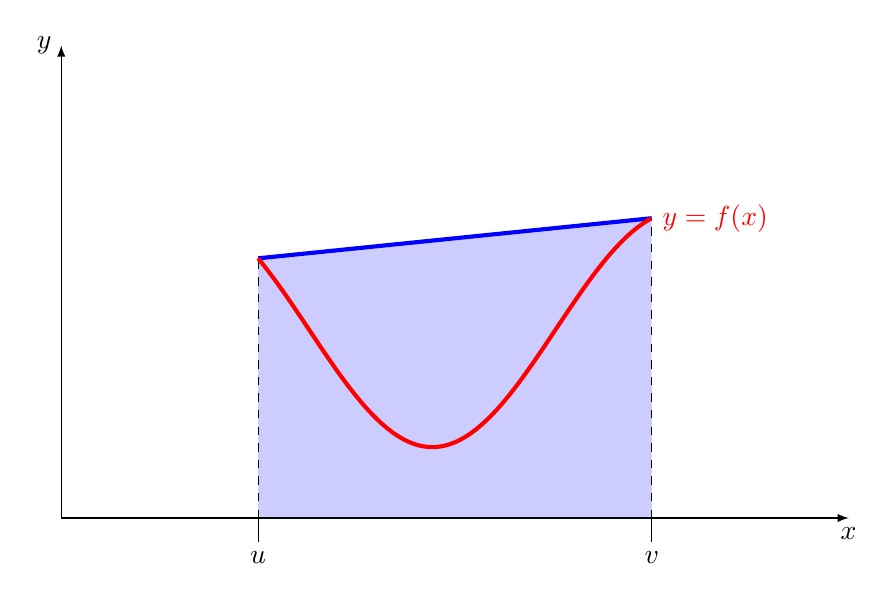
\begin{tikzpicture}[xscale=5, yscale=3]

        % Area under the affine approximation
        \fill[blue!20, domain=0.5:1.5, variable=\x]
            (0.5,0)
            -- plot ({\x}, {0.8+0.5*sin(deg(2.5)) + (\x-0.5) * 0.5 * (sin(deg(7.5)) - sin(deg(2.5)))})
            -- (1.5,0)
            -- cycle;
        % Dotted vertical line
        \draw[dashed] (0.5,0) -- (0.5, {0.8+0.5*sin(deg(2.5)});
        \draw[dashed] (1.5,0) -- (1.5, {0.8+0.5*sin(deg(7.5)});

        % axis
        \draw[-latex] (0,0) -- (2,0) node[below] {$x$};
        \draw[-latex] (0,0) -- (0,2) node[left] {$y$};
        \draw (0.5,0) -- (0.5,-0.1) node[below] {$u$};
        \draw (1.5,0) -- (1.5,-0.1) node[below] {$v$};


        % Affine approximation
        \draw[blue, line width=1.5pt, domain=0.5:1.5] plot ({\x}, {0.8+0.5*sin(deg(2.5)) + (\x-0.5) * 0.5 * (sin(deg(7.5)) - sin(deg(2.5)))});
        % Curve
        \draw[red, line width=1.5pt, domain=0.5:1.5, samples=100] plot (\x, {0.8+0.5*sin(deg(5*\x))}) node[right] {$y=f(x)$};
    \end{tikzpicture}
    \caption{Méthode du trapèze}
    \label{fig:trapeze-method}
\end{figure}

\subsection{Méthode composite du trapèze}


\quessques Écrire une fonction \texttt{trapeze\_composite(f, a, b, n)} qui calcule l'approximation de l'intégrale de \texttt{f} entre \texttt{a} et \texttt{b} pour la méthode du trapèze composite, avec une subdivision de taille \texttt{n}.
\ssques Calculer l'erreur avec la même fonction test qu'avant, pour des subdivisions de taille $ 10 $, $ 100 $ et $ 1000 $. Comparez avec les méthodes précédentes.

\begin{figure}[h!]
    \centering
    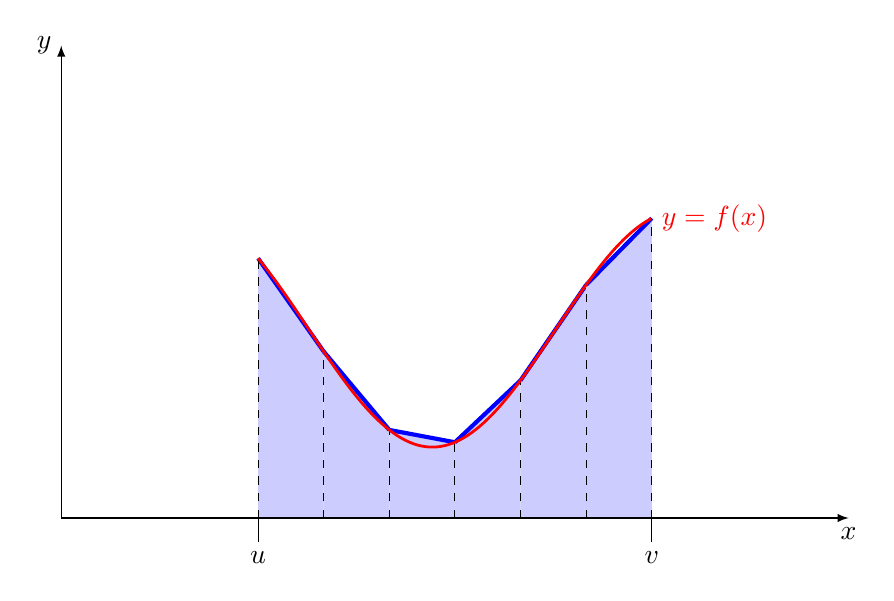
\begin{tikzpicture}[xscale=5, yscale=3]
        % Subdivisions and affine approximations
        \foreach \i in {0,1,2,3,4,5} {
            \pgfmathsetmacro{\xa}{0.5 + \i*(1/6)}
            \pgfmathsetmacro{\xb}{0.5 + (\i+1)*(1/6)}
            \fill[blue!20, domain=\xa:\xb, variable=\x]
                (\xa,0) -- plot ({\x}, {0.8+0.5*sin(deg(5*\xa)) + (\x-\xa) * 3 * (sin(deg(5*\xb)) - sin(deg(5*\xa)))}) -- (\xb,0) -- cycle;
            \draw[blue, line width=1.5pt, domain=\xa:\xb] plot (\x, {0.8+0.5*sin(deg(5*\xa)) + (\x-\xa) * 3 * (sin(deg(5*\xb)) - sin(deg(5*\xa)))});
            \draw[dashed] (\xa,0) -- (\xa, {0.8+0.5*sin(deg(5*\xa))});
            \draw[dashed] (\xb,0) -- (\xb, {0.8+0.5*sin(deg(5*\xb))});
        }

        % Axis and ticks
        \draw[-latex] (0,0) -- (2,0) node[below] {$x$};
        \draw[-latex] (0,0) -- (0,2) node[left] {$y$};
        \draw (0.5,0) -- (0.5,-0.1) node[below] {$u$};
        \draw (1.5,0) -- (1.5,-0.1) node[below] {$v$};

        % Curve
        \draw[red, line width=1.pt, domain=0.5:1.5, samples=100] plot (\x, {0.8+0.5*sin(deg(5*\x))}) node[right] {$y=f(x)$};

    \end{tikzpicture}

    \caption{Méthode composite du point milieu}
    \label{fig:trapeze-composite-method}
\end{figure}


\section{Généralisation}

Les méthodes du rectangle et du point milieu considérent que $ f $ est un polynôme de degré $ 0 $ entre les bornes. La méthode du trapèze considère que $ f $ est un polynôme de degré $ 1 $. Il est naturel de continuer ainsi pour des degrés supérieurs. La méthode suivante est celle de \textsc{Simpson}, qui approxime donc $ f $ par son interpolée de \textsc{Lagrange} en $ u $, $ \frac{u+v}{2} $ et $ v $. On peut alors montrer que cette interpolation conduit à l'approximation de l'intégrale \[
    \hat{I}_{u, v}(f) = (v-u) \cdot \left(\alpha_0 f(u) + \alpha_1 f(\frac{u+v}{2}) + \alpha_2 f(v)\right)
\]
avec $ \alpha_0=\alpha_2=\frac{1}{6} $ et $ \alpha_1=\frac{4}{6} $. On pourrait s'attendre à ce que la méthode de Simpson soit d'ordre $ 2 $, mais elle est en fait d'ordre $ 3 $, ce qui la rend encore meilleure.

En fait, chacune des méthodes que nous avons étudiées sont des cas particuliers des méthodes de \textsc{Newton-Côtes}, basées sur l'interpolation de Lagrange de $ f $ pour des partitionnements régulièrement espacés de $ [u, v] $. Même si en théorie les méthodes d'ordre supérieures fournissent une meilleure approximation de $ I(f) $, elles souffrent plus fortement des erreurs d'approximation machine dues au fait que les ordinateurs ne manipulent pas des réels mais des approximations des réels (dits \textit{nombres flottants}). En pratique, la méthode de \textsc{Simpson} est un bon compromis et la plus utilisées des méthodes de \textsc{Newton-Côtes}.

\section{Bornes sur les erreurs d'approximation}

Pour quantifier les comparaisons qualitatives entre les différentes méthodes vues jusqu'ici, on donne les bornes suivantes sur les erreurs d'approximation.
Si $ f $ est une fonction de classe $ \C^4 $ sur $ [a, b] $, notons \[
    \begin{cases}
        M_1 = \sup_{[a, b]} |f'|\\
        M_2 = \sup_{[a, b]} |f''|\\
        M_3 = \sup_{[a, b]} |f^{(3)}|\\
        M_4 = \sup_{[a, b]} |f^{(4)}|\\
    \end{cases}
\]

Alors les erreurs d'approximation ont les bornes suivantes 
\begin{align*}
    |E_{u,v}(f)| &\leq M_1 \frac{(v-u)^2}{2} \quad &&\textrm{pour la méthode du rectangle}\\
    |E_{u,v}(f)| &\leq M_2 \frac{(v-u)^3}{24} \quad &&\textrm{pour la méthode du point milieu}\\
    |E_{u,v}(f)| &\leq M_2 \frac{(v-u)^3}{12} \quad &&\textrm{pour la méthode du trapèze}\\
    |E_{u,v}(f)| &\leq M_4 \frac{(v-u)^5}{2880} \quad &&\textrm{pour la méthode de Simpson}\\
\end{align*}


\ques En déduire une borne sur l'erreur des généralisations composites avec une subdivision de taille $ n $, pour chacune des méthodes précédentes.
